\section{System API}
\label{chapAPI}
Die System API dient als Schnittstelle zum Benutzer bzw. zur Benutzerin. Dabei ist eine saubere Trennung zwischen BenutzerInnen Schnittstelle und Betriebssystem zwingend notwendig.

\subsection{Aufbau eines Systemcall Datenpakets}
Jedem Systemcall werden Daten mitgegeben, dieses müssen zuvor in eine geeignete Datenstruktur transformiert werden. In Listing \ref{systemcall-datapackage} ist die gewählte Datenstruktur abgebildet.


\lstinputlisting[language=C, caption=Aufbau eines Systemcall Datenpakets, captionpos=b, label=systemcall-datapackage]{chapters/systemapi/codefiles/datapackage.c}

\subsection{Vorgehensweise bei einem Systemcall}
Das Vorgehen bei einem Systemcall ist in Abbildung \ref{fig:Sequencediagram-systemcall} ersichtlich. 

\begin{figure}[H]
	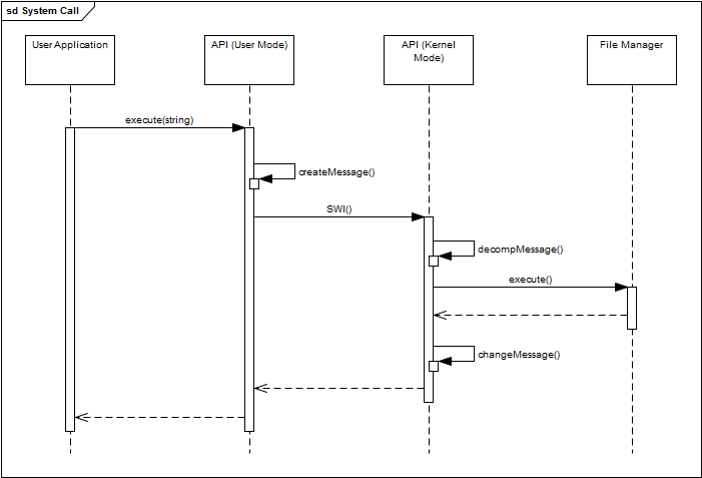
\includegraphics[scale=0.70]{chapters/systemapi/figures/systemcall-sequence-diagram}
	\caption{Sequenzdiagramm eines Systemcalls}
	\label{fig:Sequencediagram-systemcall}
\end{figure}

\pagebreak 